\newpage
\section{Introducing Algebraic Varieties}
\lecture{2}{February 15, 2021}{Varieties in RR}

\subsection{Definition}

\begin{defn}[Affine hypersurface]
	Let $K$ be a field. $K[x_1, \dots, x_n]$ is the ring of polynomials with coefficients in $K$, and 

	Suppose $p \in K[x_1, \dots x_n]$ and $p$ is not constant. Then, \[
		V(p) := \left\{(k_1, \dots, k_n) \in K^n \mid p(k_1, \dots, k_n) = 0 \right\}
	\] 
\end{defn}

\begin{exmp}
	Let $K = \RR$ and $n = 2$. Consider $p(x_1, x_2) = x_1^2 + x_2^2 - 1$. In this case, \[
		V(p) = \{(r_1, r_2) \in \mathbb{R}^2 \mid r_1^2 + r_2^2 - 1 = 0\}.
	\]

	In this case, $V(p)$ represents a circle.

	More generally, ellipses, hyperbolas, parabolas are all $V(p)$, for the right choice of $p$.
\end{exmp}

\begin{defn}[Algebraic variety]
	More generally, if $\mathcal{P}$ is a collection of polynomials in $K[X]$, not constants. Define \[
		V(\mathcal{P}) = \{(k_1, \dots, k_n) \in K^n \mid p(k_1, \dots, k_n) = 0, \forall p \in \mathcal{P}\}.
	\] 
\end{defn}

\subsection[Examples in real numbers]{Examples with $K = \RR$}

\begin{ques}
	What sorts of geometric properties can algebraic varieties have?
\end{ques}

\begin{exmp}
	Consider $p(x, y) = y^2 - x^3$.  Then, $V(p)$ looks like:
	\begin{center}
		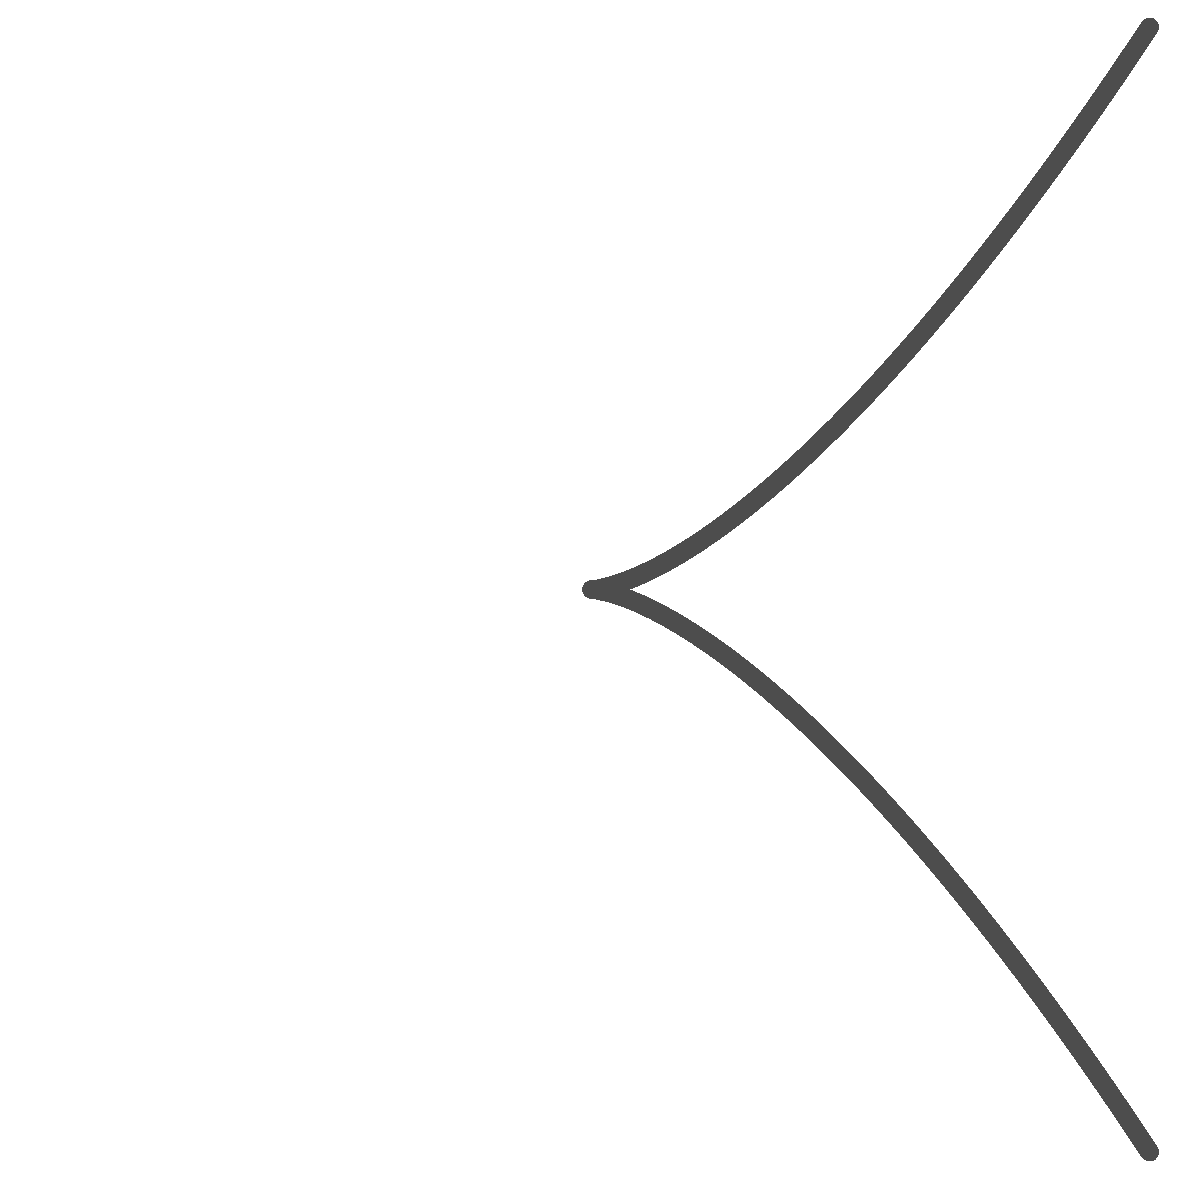
\includegraphics[width = .25\textwidth]{figures/variety_example_1.pdf}
	\end{center}
\end{exmp}

\begin{exmp}
	Consider $q(x, y) = y^2 - x(x^2 - 1)$. Then,  $V(q)$ looks like:
	\begin{center}
		\includegraphics[width = .25\textwidth]{figures/variety_example_2.pdf}
	\end{center}
\end{exmp}

\begin{exmp}
	Consider $r(x, y) = y^2 - x^2(x+1)$. Then, $V(r)$ looks like:
	\begin{center}
		\includegraphics[width = .25\textwidth]{figures/variety_example_3.pdf}
	\end{center}
\end{exmp}

\begin{exmp}
	Consider $s(x, y) = xy$. Then, $V(s)$ looks like:
	\begin{center}
		\includegraphics[width = .25\textwidth]{figures/variety_example_4.pdf}
	\end{center}
\end{exmp}

\begin{defn}
	We say a variety has dimension $d$ if a subset of it ``looks like $\mathbb{R}^d$'' and if it is the disjoint union of finitely many pieces that each ``look like  $\mathbb{R}^i$'' with $0 \le i \le d$
\end{defn}

\begin{exmp}
	The dimension of $V(x^2 + y^2 - 1)$ is $1$.
\end{exmp}

\begin{exmp}
	The dimension of $V(\{x, y\}) = \{(0, 0)\}$ is $0$.
\end{exmp}

In Linear Algebra, the number of linearly independent always equals the codimension of the solution set.

\begin{ques}
	Does this hold for varieties?
\end{ques}
\begin{ans}
	No. $V(x^2 + y^2) = \{(0, 0)\}$, which has dimension $0$ (as opposed to the expected $2 - 1 = 1$). Another example is $V(y, y - 1) = \varnothing$, which has dimension $-1$ (as opposed to the expected $2 - 2 - 2$).
\end{ans}

So, linear algebraic dimension count fail for varieties for at least two reasons:
\begin{enumerate}[label = \textbullet]
	\item non-existence of solutions to certain types of algebraic equations (e.g., $x^2 = - 1$).
	\item non-extistence of intersections between parallel lines.
\end{enumerate}
